% fig_protocol_stack.tex — Pre-compiled TikZ figure (Overleaf version)
\begin{figure}[H]
\centering
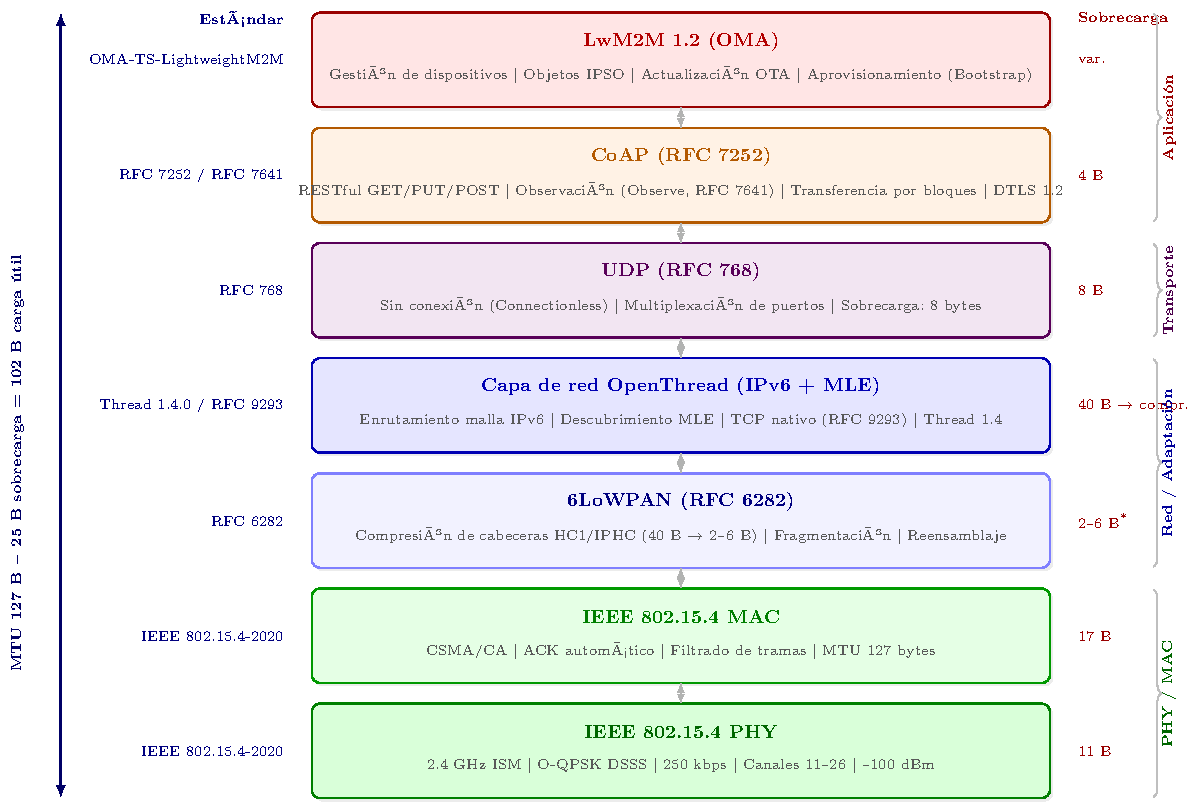
\includegraphics[width=\textwidth]{tikz_pdfs/fig_protocol_stack.pdf}
\caption{Pila completa de protocolos de comunicación para nodos IoT Thread/LwM2M. La arquitectura implementa 7~capas desde IEEE~802.15.4 PHY (capa física 2,4\,GHz, 250\,kbps) hasta LwM2M~1.2 (gestión de dispositivos). OpenThread proporciona red IPv6 en malla auto-configurable sobre IEEE~802.15.4 con soporte TCP nativo (RFC~9293), con 6LoWPAN comprimiendo cabeceras IPv6/UDP/TCP (60~bytes $\rightarrow$ 6--12~bytes típico) para maximizar la carga útil. CoAP implementa RESTful sobre UDP con extensiones de observación (Observe, RFC~7641) para notificaciones asíncronas. LwM2M aprovecha CoAP para operaciones CRUD sobre objetos estandarizados (IPSO Smart Objects), habilitando gestión remota, actualización OTA y aprovisionamiento automático. MTU efectivo: 127~bytes MAC $-$ 25~bytes de sobrecarga = 102~bytes de carga útil disponible para datos de aplicación.}
\label{fig:protocol-stack}
\end{figure}
